\documentclass[12pt]{report}
\usepackage{cuthesis}
\usepackage{amsmath}
\usepackage[font=small,format=plain,labelfont=bf,up,textfont=up]{caption}
\usepackage[T1]{fontenc}
\usepackage{graphicx}
\usepackage{subfigure}
\usepackage{float}
\usepackage{listings}
\usepackage{courier}
\usepackage[ruled,vlined]{algorithm2e}
\usepackage{verbatim}
\usepackage[toc, page]{appendix}

\author{Guangfu Shi}
\title{Efficient Global Illumination Techniques On GPU}
\degree{Master of Computer Science}
\dept{Computer Science}       						% default is Comp.Sci.
%\cosupervisor{Dr. Thomas Fevens}                   	% if you also have a co-supervisor


% Source Code Formatting
\lstset{
         %basicstyle=\footnotesize\ttfamily, % Standardschrift
         basicstyle=\small\ttfamily,
         %numbers=left,               % Ort der Zeilennummern
         numberstyle=\tiny,          % Stil der Zeilennummern
         %stepnumber=2,               % Abstand zwischen den Zeilennummern
         numbersep=5pt,              % Abstand der Nummern zum Text
         tabsize=2,                  % Groesse von Tabs
         extendedchars=true,         %
         breaklines=true,            % Zeilen werden Umgebrochen
         keywordstyle=\color{red},
         %frame=t|b,         
 %        keywordstyle=[1]\textbf,    % Stil der Keywords
 %        keywordstyle=[2]\textbf,    %
 %        keywordstyle=[3]\textbf,    %
 %        keywordstyle=[4]\textbf,   \sqrt{\sqrt{}} %	
         stringstyle=\color{white}\ttfamily, % Farbe der String
         showspaces=false,           % Leerzeichen anzeigen
         showtabs=false,             % Tabs anzeigen ?
         xleftmargin=17pt,
         framexleftmargin=17pt,
         framexrightmargin=5pt,
         framexbottommargin=4pt,
         %backgroundcolor=\color{lightgray},
         showstringspaces=false      % Leerzeichen in Strings anzeigen ? 
         captionpos=b
 } 


%---- Set figures path ----
\graphicspath{{C:/Users/steve-laptop-M4600/develop/projects/master_thesis/thesis/imgs/}}

\begin{document}

\begin{abstract}
  Text of abstract.  
\end{abstract}

\begin{acknowledgments}
  Text of acknowledgments.
\end{acknowledgments}

%%%%%%%%%%%%%%%%%%%%%%%%%%%%%%%%%%%%%%%%%%%%%%%%%%%%%%%%%%%%%%%%%%%%%%%%%%%%%%%
%% Body of Thesis goes here.
%%%%%%%%%%%%%%%%%%%%%%%%%%%%%%%%%%%%%%%%%%%%%%%%%%%%%%%%%%%%%%%%%%%%%%%%%%%%%%%

% Set the page numbering style
\pagenumbering{arabic}
\setcounter{page}{1}
	
%------------------------
% Chapter 1 : Introduction	(2 p)
\chapter{Introduction}

\section{Problem Statement}

Recently, with the dramatically boost of computing power of the current generation Graphics Processor Unit (GPUs) device, the application of the massive parallel computing capability offered by GPU has been drawn more and more interest in the field of Computer Graphics, especially realistic image synthesis.  

Realistic image synthesis technique has always been known computing power demanding due to the physically based simulations. In order to produce images with decent quality and handle wider range of types of materials in the scene, solving the Light Transport  Equation (LTE) require more effort such as accelerating of ray-object intersections query, more sampling of the ray path and multi-pass rending technique. However, it is not free to take the advantage of GPUs' processing power, algorithms have to be parallelized to be suitable of hardware and the programmers is required to code carefully to make sure to follow the best practice of programming on GPU. 

An example of the algorithm parallelization is the construction of KD-Tree acceleration structure for both scene objects (triangles) and photons(points). The algorithm is designed in Breadth First style using GPU instead of the Depth First style using CPU. The data structure is also implemented in Structure of Arrays (SoA) on GPU instead of Array of Structures (AoS) to fit the GPU memory access pattern. 

Adapt the program to be be GPU hardware friendly is also challenging. For example, irregular memory access on GPU can be huge performance overhead, smart utilization of the memory hierarchy (such as the using the shared memory over global memory) on GPU is very helpful to hide memory latency. 

\section{Structure of the Thesis}	


%-------------------------
% Chapter 2:  Background	(~10 p)
%- Radiometry Introduction.
%- Rendering equation. 
%- LTE equation 
%- BRDF 
%- Monte-Carlo Ray Tracing. 
%- Russian roulette
\chapter{Background}

To establish the mathematics basis and mental model of the problem, some essential conceptions in Computer Graphics are going to be introduced in this chapter.  

%%%%%%%%%%%%%%%%%%%%%%%%%%%%%%%%%%%%%%%%%%%%%%%%%%%%%%%%%%%%%%%%%%%%%%%%%%

\section{Radiometry Introduction}
Radiometry is the basic terminology to describe light which is crucial to simulation. First of all, some basic quantities have to be introduced, the related symbols are going to be defined here as well for further use.

\subsection{Important Quantities} 

\begin{table}[!ht]
\begin{center}
	\begin{tabular}{ | l | l | l |}     	
	\hline 

	Symbol & Quantity & Unit \\

	% \(Q_{\lambda}\) 	& 		Spectral radiant energy 		& 		\(J nm^{-1} \) \\
	\(Q\) 			& 		Radiant Energy 				& 		\(j\) \\ 
	\(\Phi\) 			& 		Radiant flux 					& 		\(W\) \\ 
	\(I\) 			& 		Radiant intensity 				& 		\(W sr^{-1}\) \\
	\(E\)			&		Irradiance (incident) 			&		\(W m^{-2}\) \\  
	\(L\)			&		Radiance						&		\(W m^{-2} sr^{-1}\) \\ 
	
	\hline

	\end{tabular}
\end{center} 
\caption{Radiometric symbols, names and units.}
\label{tab:radiometry_quantities}
\end{table}

\emph{Radiant energy}, \(Q\), is the energy of a collection of photons which is the basic quantity in lighting. 

\emph{Radiant flux} , \(\Phi\), is the time rate of the flow of radiant energy passing through a surface or region of space. Total emission from a light source is generally described in terms of flux. \ref{fig:flux_point_light} shows the flux emitted from a point light source measured by the total amount of energy passing through an virtual sphere around the light. 

\begin{figure}[htp] 
    \centering 
    \fbox{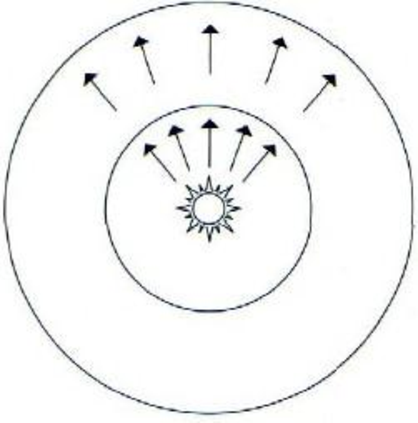
\includegraphics{flux.pdf}}
    \renewcommand{\thefigure}{\thechapter.\arabic{figure}}
    \caption[]{Radiant flux from a point light source is passing through the spheres around the light.}
    \label{fig:flux_point_light} 
\end{figure} 

\emph{Irradiance}, \(E\), is the incident (arriving at a surface location) \emph{radiant flux area density}, which is defined as the differential flux per differential area. While \emph{Radiant exitance} denoted by \(M\) is area density of flux leaving a surface.  

\begin{equation}
E(x) = \frac{d\Phi}{dA}
\end{equation}

\emph{Radiance}, \(L\), is the radiant flux per unit solid angle per unit projected area: 

\begin{equation}
L(x, \overrightarrow{\omega}) = \frac{d^{2}\Phi}{\cos{\theta} \cdot dA \cdot d\overrightarrow{\omega}}
\end{equation}

Where \(x\) is the position and \(\overrightarrow{\omega}\) is the direction. 

Radiance is the most important quantity in rendering simulation since it closely represent the color. Also radiance can be considered as the number of photons arriving per time at a small area from a given direction. Radiant energy can be computed by integrating the radiance field over all directions \(\Omega\) and area \(A\).

\begin{equation} 
\Phi = \int_{A}\int_{\Omega}L(x, \overrightarrow{\omega})(\overrightarrow{\omega} \cdot \overrightarrow{n})d\overrightarrow{\omega}dx
\label{eq:flux_from_radiance}
\end{equation} 

\begin{figure}[htp] 
    \centering 
    \fbox{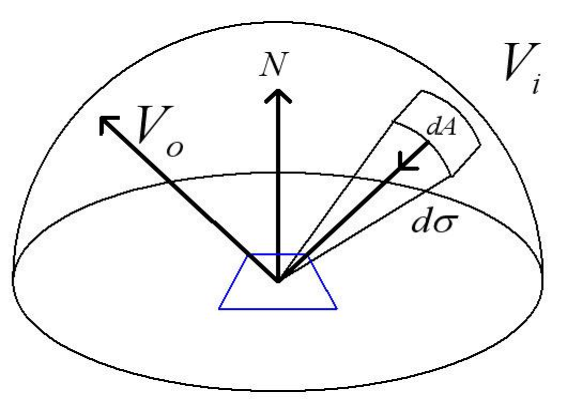
\includegraphics{solid_angle_sphere.pdf}}
    \renewcommand{\thefigure}{\thechapter.\arabic{figure}}
    \caption[]{Radiance, L, is defined as the radiant flux per unit solid angle, \(\overrightarrow{\omega}\), per unit projected area, \(dA\)}
    \label{fig:solid_angle_sphere} 
\end{figure}

The solid angle used in equation \ref{eq:flux_from_radiance} can be thought as representation of both a direction and an infinitesimal area. Therefore solid angle can also be expressed in spherical coordinates (\(\theta, \phi\))

\begin{figure}[htp] 
    \centering 
    \fbox{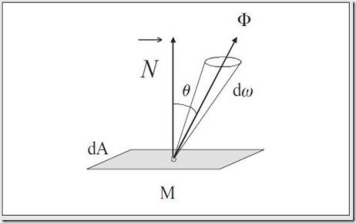
\includegraphics{radiance_solid_angle.pdf}}
    \renewcommand{\thefigure}{\thechapter.\arabic{figure}}
    \caption[]{Radiance, L, is defined as the radiant flux per unit solid angle, \(\overrightarrow{\omega}\), per unit projected area, \(dA\)}
    \label{fig:radiance_solid_angle} 
\end{figure} 

\subsection{Light Source}
The light in the form of photons is emitted from light sources. We can measure the intensity of light source in \emph{wattage}. Take a point light source for example, the power this light can emit is denoted by \(\Phi\), the emitted light distribute uniformly in all directions, the irradiance, \(E\), can be computed at a surface as: 

\begin{equation}
E(x) = \frac{\Phi \cos{\theta}}{4\pi r^{2}} 
\end{equation}

Where \(r\) is the distance from \(x\) to the light source and \(\theta\) is the angle between the surface normal and the direction to the light source. From the equation we can intuitively tell a surface facing the source will receive more photons per area than a surface that is oriented differently.   

%%%%%%%%%%%%%%%%%%%%%%%%%%%%%%%%%%%%%%%%%%%%%%%%%%%%%%%%%%%%%%%%%%%%%%%%%%


\section{Render Equation}
With the physically-based model of lighting, a theoretical framework describing the interaction between light and an surface will be introduced in this section. 

\begin{figure}[htp] 
    \centering 
    \fbox{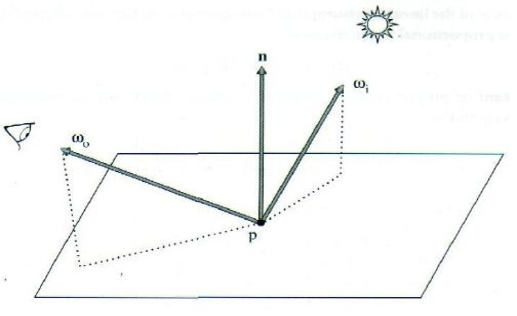
\includegraphics{brdf.pdf}}
    \renewcommand{\thefigure}{\thechapter.\arabic{figure}}
    \caption[]{The geometric setup of BRDF. }
    \label{fig:brdf} 
\end{figure} 

The \emph{Bidirectional Reflectance Distribution Function}, BRDF, is the mathematic tool describing the reflectiona of light encounters an surface. To define the BRDF, the geometric configuration is shown in figure \ref{fig:brdf}. \(\omega_{i}\) is the incident lighting direction, \(\omega_{o}\) is the direction in which the reflected light leaving from the surface, \(n\) is the normal vector at the location \(p\) on the surface. Given the incident radiance \(L_{i}(p, \omega_{i})\), we are finding out the outgoing radiance to the viewer, \(L_{o}(p, \omega_{o})\). 

The BRDF, \(f_{r}\), defines the relationship between differential reflected radiance and differential irradiance: 

\begin{equation}
f_{r} = \frac{dL_{o}(p, \omega_{o})}{dE(p, \omega_{i})} = \frac{dL_{o}(p, \omega_{o})}{L_{i}(p, \omega_{i})(\omega_{i} \cdot n)d\omega{i}}
\label{eq:brdf}
\end{equation} 

There are two important properties of BRDF used in rendering. The first one is the Helmholtz's law of reciprocity, that is given any pair of directions \( (\omega_{i}, \omega_{o} ) \), we have: 

\begin{equation}
f_{r}(p, \omega_{i}, \omega_{o}) = f_r(p, \omega_{o}, \omega_{i})
\end{equation}

Another important physical property of BRDF is energy conservation, stating that the total reflected energy is less than or equal to the incident energy. For all direction \( \omega_{o} \).

\begin{equation}
 \int_{\Omega}f_{r}(p, \omega_{i}, \omega_{o})L_{i}(p, \omega_{i})(\omega_{i} \cdot n)d\omega_{i} \leq 1 , \forall \omega_{i}
\end{equation}

Given the definition of BRDF, we can introduce the basic render equation, also known as \emph{local illumination model} by integrating the equation \ref{eq:brdf} over the sphere of incident directions around location \(p\), the left side of the equation will be the outgoding radiance in direction \(\omega_{o}\).

\begin{equation}
L_{o}(p, \omega_{o}) = \int_{\Omega}f_{r}(p, \omega_{i}, \omega_{o})L_{i}(p, \omega_{i})(\omega_{i} \cdot n)d\omega_{i}
\label{eq:local_render_equation}
\end{equation}

Where \(\Omega\) is the hemisphere of incoming directions at \(p\).

\paragraph{Light Transport Equationa} 

The local illumiation model is used to describe the direct lighting effect which is too simple for simulating real-world lighting effect, indirect lighting has to be introduced to this model as well. Therefore we introduce the Light Transport Equation (LTE) in this section to form the mathematical basis for all global illumination algorithms, The LTE states the necessary conditions for equilibrium of light transport in the scene without participating media. 

\begin{equation}
L_{o}(p, \omega_{o}) = L_{e}(p, \omega_{o}) + \int_{\Omega}f_{r}(p, \omega_{i}, \omega_{o})L_{i}(p, \omega_{i})(\omega_{i} \cdot n)d\omega_{i}
\label{eq:lte}
\end{equation}

%%%%%%%%%%%%%%%%%%%%%%%%%%%%%%%%%%%%%%%%%%%%%%%%%%%%%%%%%%%%%%%%%%%%%%%%%%

\section{Monte-Carlo Ray Tracing} 




%-------------------------
% Chapter 3: Global Illumination and Photon-mapping using GPU 	(~10 p) 
%- KD-Tree Construction and representation on GPU
%- Photons KNN search using KD-Tree
%- Selective sampling 
%- New algorithm: localized update the photons 
\chapter{A New Approach}

In this chapter, we will present a noval approach for rendering a scene with dynamic light source efficiently. This method is based d on the standard GPU-based photon mapping rendering system, using an augmented kd-tree data structure and localized updating algorithm for rendering.  

In the first 2 sections of this chapter, We will have an overview on our approach and comprehensive description of the data structure that we use and related algorithms. Then we will look at some of the GPU implementation details. 

\section{Overview} 

As described in chapter 2, we build a gloabl kd-tree as the photon map for irradiance estimation. However, the global photon map is rebuilt from scratch every frame, this process is time consuming due to the complexity of kd-tree building algorigthm on GPUs and can be avoided. 

Instead of building a global kd-tree for photons, we re-use the same kd-tree for the geometry objects(triangles) which is static and associate the geometry and the photons data for efficient KNN search and update for dynamic scene. 

For each frame, the photons are shot from the light source and stored in an array, then we build the kd-tree for the geometry objects if it is required, for the scenes that don't include animated objects we will skip this process. Given the photons data in the scene and the built kd-tree for geometry, we build our data structure, compress the memory bind it to the texture memory for a better memory accessing performance. In rendering phase, instead of using photon map for radiance estimation, we use the kd-tree and our photon queue perform KNN search. Further details of the data structure will be presented in the following section. 

The update process of photons queue is straightforward. It depends on the photon data from the previouse frames. Here we keep track of all the photons data of a range of frames with a pair of indices, the indices can be updated and maintained efficiently. Furthur  details will be presented in following section.  

\section{Data Structure And Algorithm} 

\subsection{Data Structure}

\begin{figure}[htp] 
    \centering 
    \fbox{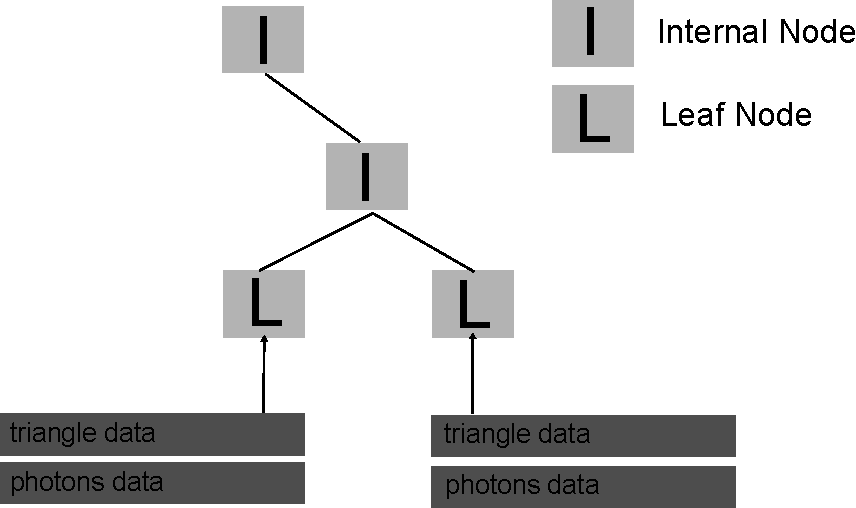
\includegraphics{imgs/kd_leaf_photons.pdf}}
    \renewcommand{\thefigure}{\thechapter.\arabic{figure}}
    \caption[]{Radiant flux from a point light source is passing through the spheres around the light.}
    \label{fig:kd_leaf_photons} 
\end{figure}  

As shown in figure \ref{fig:kd_leaf_photons}, in addition to the triangle data, the photons data in the scene is also logically associated with the leaf nodes of the kd-tree. As the kd-tree for the scene actually encodes the spatial relationship among the geometry, and the photons will be stored when they hit the objects with diffuse objects, we attach the photons fall into the spatial region occupied by the bouding box of a kd-tree leaf node. 

\begin{figure}[htp] 
    \centering 
    \fbox{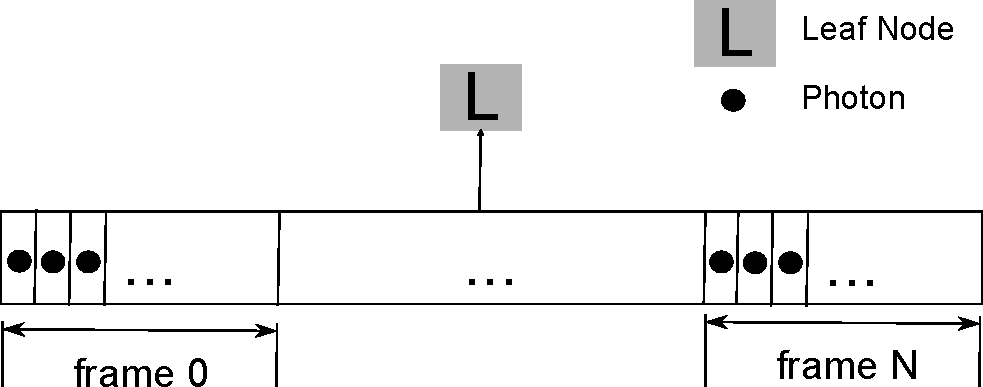
\includegraphics[width=\linewidth]{imgs/kd_leaf_photons_2.pdf}}
    \renewcommand{\thefigure}{\thechapter.\arabic{figure}}
    \caption[]{Radiant flux from a point light source is passing through the spheres around the light.}
    \label{fig:kd_leaf_photons_2} 
\end{figure}  

In figure \ref{fig:kd_leaf_photons_2} we have a more detailed view on how the photons data organized. The photons shot to the scene in one frame of rendering are stored followed by the photons of next frame. When implementing this organization on GPU, all actual photons data (positions, incident directions and power) is stored in a seperate array, the indices of the photons associated with kd-tree leaf nodes are stored instead of the actual photon data. 

\subsection{Construction} 

Building the logical connection between photons and leaf nodes is simpler than build a global kd-tree for the photon map. Firstly, we found out the the leaf nodes from the built kd-tree in parallel. This can be done checking a flag set when building the kd-tree. Given the indices of leaf nodes, we can retrieve the bounding box from the small node list generated in kd-tree construction phase(see \ref{subsec:kdtree_construction}). Then we check which leaf node certain group of photons should fall into in parallel by performaing fast point-box intersection testing. For each leaf node, the number of photons can be calculated with a parallel reduction operation. Further details on physical memory arrangement and implementation of the data structure  will be presented in section \ref{sec:impl_detials}. 

\subsection{Update} 

When a frame of image is rendered, new photons will be shot into the scene and be stored in the same global array with previous frames and for each leaf node, we need to keep track of the range of the photons that are active for rendering the next frame. For each leaf node, we maintain two pointers(indices), start and end index, indicating the range of the photons used for rendering. We move the end pointer forward as there are new photons comming, move the start pointer forward when there are some old photons we need to discard. We use a pre-defined threshold fram count to determine how manay frames of photons data we want to make active, we keep accumulating the photons every frame until we reach that threshold value. When the threshold frame count 
is reached, we move forward the start pointer to avoid there are too many photons than there should be. Since the number of photons per frame is known, the stride of moving start pointer can be calculated. However, in GPU implementation, the step in bytes used to increment the pointer is usually larger than the exact size of photons data we want to discard, since the memory will be padded when it is allocated for better memory accessing performance. Further details will be presented in section \ref{sec:impl_detials}. 

\subsection{Rendering} 

Rendering with our data structure does not differ much from the standard photon mapping rendering algorithm. In rendering phase, we cast the rays from the camera into the scene in parallel and perform KNN search using the kd-tree already built for the geometry, when we reach the leaf nodes we use our data structure to find the photons data for particular leaf node and gather the photons for radiance estimation. 

\section{Implementation Details} 
\label{sec:impl_detials} 

\subsection{Data Organization} 
\label{subsec:data_org}

\paragraph{KD-Tree Data} 

The kd-tree data should be carefully organized when implemented with CUDA to improve traversal performance. In \ref{subsec:kdtree_construction}, we have already described the kd-tree building algorithm introduced in \cite{Zhou2008}, but some of the details that are critical to the program's overall performance still need to be discussed here. 

The final node list generated when the kd-tree is built is not sufficient for fast traversal algorithm, it contains too much useless information and will hit the performance since it is not friendly to cache prefetch. Therefore we compress and re-organize the traversal related data of the kd-tree nodes to reduce the memory access. The entire kd-tree is stored in a structure of several contiguous arrays. The structure is defined as following:  

% Code Snippet
\lstinputlisting{kdtree_data_def.cpp} 

The traversal data is compressed into an unsigned integer array, as shown in the following figure: 

\begin{figure}[htp] 
    \centering 
    \fbox{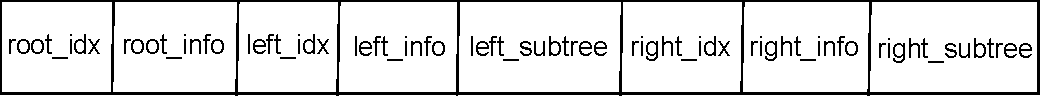
\includegraphics[width=\linewidth]{imgs/kdtree_data_memory_layout.pdf}}
    \renewcommand{\thefigure}{\thechapter.\arabic{figure}}
    \caption[]{Compacted kd-tree data memory layout.}
    \label{fig:kdtree_data_memory_layout} 
\end{figure}  

Where root\_info, left\_info and right\_info are the parent information for the root, left and right child node(if left and right node are inner nodes). This is a compressed form of what is needed during kd-tree traversal. Parent information stores two unsigned integers, hence two elements in the d\_preorder\_tree array. The first unsigned integer contains several information of the inner node: the split axis takes 2 most significant bits and address of right node in the d\_preorder\_tree array, which is 0 if it is a leaf node, take the rest bits. The second unsigned integer stores the split position(a float value stored as unsigned integer). The address of left child node is not stored explicitly as it can be computed by skipping the parent info(2 unsigned integers) from current node's address. The 2 bits for split axis can represent \(x\) axis if it is 0, \(y\) axis if it is 1 and \(z\) axis if it is 2. 

Where the root\_idx, left\_idx and right\_idx are the indices of the root, left and right nodes. The indices can be used to access the other arrays such as the node extents array. The type information of the nodes is also encoded in the indices, if it is a leaf node, the most significant bit(MSB) is set, else the MSB is not set, this improves leaf detection performance because it avoids reading child information. The above format applies only for inner nodes, for leafs, instead of parent information, element count and element indices are stored. The element indices are relative to the underlying triangle data. Hence we have the following format: 

\begin{figure}[htp] 
    \centering 
    \fbox{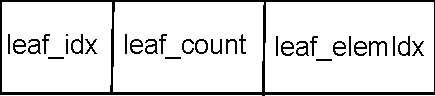
\includegraphics{imgs/kdtree_data_memory_layout_2.pdf}}
    \renewcommand{\thefigure}{\thechapter.\arabic{figure}}
    \caption[]{Compacted kd-tree data memory layout.}
    \label{fig:kdtree_data_memory_layout} 
\end{figure}  

\paragraph{Photons Data} 


\paragraph{Connection Between KD-Tree and Photons Data} 

The connection between KD-Tree leaf nodes and photons data is stored as a structure of several data array like storing other type of data on GPU side. 

\subsection{Algorithm Description} 

\subsubsection{Construction}  

\begin{algorithm}[H]
	\SetAlgoLined
	\SetKwInOut{Input}{input}\SetKwInOut{Output}{output}
	\Input{KD-Tree Data} 
	\Input{Photons Data} 
	\Output{KD Leaf Nodes Photons List} 

	\( leafNodesMarks \leftarrow new\ array  \) \\
	\( leafNodesIndices \leftarrow new\ array  \) \\
	\( identityIndices \leftarrow (0, 1, 2 ... n) \) \\ 

	\For{All nodes of KD-Tree in parallel} {
		\( leafNodesMarks \leftarrow mark\ leaf\ nodes  \) \\
	}

	\( leafNodesIndices \leftarrow new\ array  \) \\
	\(tempArray \leftarrow \) Multiply \(identityIndices\) and \(leafNodesMarks\)
	\( leafNodesIndices \leftarrow \) Compact \( tempArray \)
	 
	\For{All KD-Tree leaf nodes in parallel} {
		\For{All photons of current frmae in serial} {
			Perform point-box intersection detection. \\ 
			Store indices of photons 
		}
	}
	
	\For{All leaf nodes of KD-Tree in parallel} {
		\If{frame counter \(<\) max frames} {
			Store photons indices of current frame with current end pointer. 
		}

		Update start and end pointer for current leaf node.
	}
	
	\caption{Classify photons to kd-tree leafs. } 	
	\label{algo:build_kdleaf_photons} 
\end{algorithm}

 \vspace{20pt}

In algorithm \ref{algo:build_kdleaf_photons}, it takes two major pieces of input data, the kd-tree data constructed for the scene and the photons data shot in the scene. The photons data is updated every frame by inserting new photons to an big chunk of buffer resides in GPU memory. Similar to the organization of underlying triangle data for kd-tree nodes, the memory for each frame of photons is aligned to a fixed size to enable coalesced memory access which may improve the performance considerably. This is one of the most important good practices for CUDA programming, because if the threads in a block are aceessing consecutive memory locations, then all the accesses are combined into a single request by the hardware. However organizing data in this way will bring extra complexity for implementation because we have to keep track of the locations of beginning of next valid chunk of data for data accessing and there will be holes contained in the whole data array. Therefore move the pointer from \(i\)th frame to \(i+1\) frame requires increasing the pointer by maximum size of memory of \(i\)th frame which is aligned to a fixed size. 

We firstly mark the leaf nodes from the input kd-tree data, given the data definition described in the section \ref{subsec:data_org}, we only need to look at alll the nodes and test if the MSB of the node's index is set. The indices of nodes can be retrieved from the kd-tree data. We store the result of marks in an array with the same number of elements as number of kd-tree nodes, the result will be 1 for a leaf node and 0 otherwise. The number of leaf nodes can be calculated by performing a data parallel reduction on this array. In order to store the indices of leaf nodes into an array of our data structure, we use another temporary local array and fill it with identity values \( (0, 1, 2 ... n-1) \), where \(n\) equals to the total count of kd-tree nodes, then we use the makrs of leaf nodes as a filter to select the leaf nodes by performing an array multiplication for each elements on these two arrays, lastly we need a data parallel algorithm, compact, to remove all the invalid value(0s) from the result of previous step and store the result. 

Our goal is that connect photons with kd-tree leaf nodes so that we can easily find the photons according to the indices of leaf nodes. So we need to classify the photons into an array with the same order of the indices of leaf nodes. For example, the \(a\)th leaf node associates with a range of photons [i ... i + n]. Firstly, we launch a kernel program on all leaf nodes performing the intersection detections between the bounding box and point on all of photons, if the photon is contained in a certain leaf node, then we store the indices of photons. 

The data structure used to store photons for kd-tree leaf nodes works in the similar way to the circular buffer. We store number of frames of photons in a contiguous buffer. The start and end pointer(indices) indicate a range of frames of photons that is valid for rendering this frame. The start pointer points to the first photons of first active frame and the end pointer points to the first photon of the last active frame. We have a frame counter indicating the number of frames we have in the range, therefore we can detect if the buffer is full by compare the frame counter and max frames capacity. 


\subsubsection{Render} 

\begin{algorithm} 
	\SetAlgoLined
	\SetKwInOut{Input}{input}\SetKwInOut{Output}{output}
	\Input{Query Point} 
	\Input{Camera Rays}
	\Input{Query Radius} 
	\Input{Diffuse Colors}
	\Output{Radiance} 
	
	\For{All intersection points in parallel} {
		Retrive diffuse color at intersection point; \\
		Retrive the normal vector at intersection point; \\
		Flip the normal vector if it is needed; \\ 
		\( irradiance \leftarrow rangeSearch(intersectPoint) \); \\
		\( radiance \leftarrow colorDiffuse \cdot Pi^{-1} \cdot irradiance \); 	
	}
	\caption{Radiance estimation with kd-tree and photons queue.} 	
	\label{algo:render_kdleaf_photons} 
\end{algorithm}

Algorithm \ref{algo:render_kdleaf_photons} shows the main framework of estimating the radiance at a query point in parallel. Each CUDA thread works on one query point. The key part of this computation is performing KNN range search around the query point with the kd-tree and the photons queue as input. The KNN range search function sums up all the power(flux) of photons and output the irradiance by dividing the flux by the area of circle centered at the query with a predefined radiance. 

\begin{algorithm}
	\SetAlgoLined
	\SetKwInOut{Input}{input}\SetKwInOut{Output}{output} 
	\Input{Query point position} 
	\Input{Query radius} 
	\Input{KD-Tree Data} 
	\Input{Leaf nodes photons queue}
	\Output{Number of photons found}
	\Output{Irradianc}
	
	totalFlux \(\leftarrow\) 0; \\
	todoStack \(\leftarrow\) new\ Array[KD\_MAX\_HEIGHT]; \\
	nodeAddr \(\leftarrow\) 0; \\

	\While{\(nodeAddr >= 0\)} {

		idxNode \(\leftarrow\) kdTreeData.preorderTree[nodeAddr]; \\ 
		isLeaf \(\leftarrow\) idxNode\ \&\ 0x80000000; \\ 
		idxNode \(\leftarrow\) idxNode\ \&\ 0x7fffffff; \\ 
		
		\While{\(NOT\ isLeaf\)} {
			leftNodeAddr \(\leftarrow\) nodeAddr+1+2; \\
		
			parentInfo \(\leftarrow\) GetParentInfo(kdTreeData); \\
			splitAxis \(\leftarrow\) GetSplitAxis(parentInfo); \\ 
			splitPos \(\leftarrow\) GetSplitPos(parentInfo); \\
			rightNodeAddr \(\leftarrow\) GetRightNodeAddr(parentInfo); \\
		
			distSqr \(\leftarrow\) Sqr(queryPoint[splitAxis] \(-\) splitPos); \\ 
			
			nodeAddr \(\leftarrow\) leftNodeAddr; \\
			otherNodeAddr \(\leftarrow\) rightNodeAddr; \\
			\If{queryPoint[splitAxis] \(>\) splitPos} {
				nodeAddr \(\leftarrow\) rightNodeAddr; \\
				otherNodeAddr \(\leftarrow\) leftNodeAddr; \\
			}
			\If{ distSqr \(<\) queryDistSqr } { 
				todoStack[todoPos++] \(\leftarrow\) otherNodeAddr; \\ 
			} 
			
			Read node index + leaf info (MSB) for new node. \\
		}
		
		/* Now we have a leaf node */ \\
		photonIdx \(\leftarrow\) photonsQueue.start; \\
		numPhotons \(\leftarrow\) photonsQueue.numPhotons; \\
		\While {has more photons} {
			photonPos \(\leftarrow\) GetPhotonPos(photonIdx); \\
			pointDistSqr \(\leftarrow\) ComputeDistantSqr(queryPoint, photonPos); \\
			\If {pointDistSqr \(<\) queryDistSqr} {
				totoalFlux \(\leftarrow\) Add the flux of photons; \\
			} 
		} 
		\(nodeAddr\) \(\leftarrow\) Pop next node from next stack; \\	
	}	
	
	\Return irradiance \(\leftarrow\) totalFlux \/ maxRadiusSqr * Pi; \\ 
	
	\caption{KNN range search with kd-tree and photons queue.} 	
	\label{algo:knn_kdleaf_photons} 
\end{algorithm}

In algorithm \ref{algo:knn_kdleaf_photons}, we present the KNN range search using our data structure. The basic layout of the algorithm follows the standard while-while iterative traversal scheme.  We first allocate an array as the stack for the kd-tree traversal. Note that this array resides on the local memory of the CUDA thread running this algorithm, therefor the access to local array is always coalesced. Then we visit the kd-tree nodes in pre-order style using the compressed kd-tree data. If the current node is an internal, then we determine which subtree we will go deeper by compare the position of query point and split plane with respect to the split axis. If the other child node is in the range of search radius, it is going to be pushed to the stack. When a leaf node is reached, we look up the photons queue in which the range of photons for searching is marked by the start and end pointer and iterate over the photons finding the ones in the searching radius and calculate the irradiance. 



%-------------------------
% Chapter 4: Performance Measurement (5 p) 
\chapter{Simulation Result}

In the first section, we will have an overview on our simulation program and our testing environment. Then in the following section, the simulation results and analysis will be presented as the concept proof of our new approach. 


\section{Overview}

In this section, we will have an overview on our simulation program and our testing configuration. 

Our simulation program is implemented with CUDA, the host part of the code is fully written in C++ and the code running by GPU is written in CUDA C which is an extension of standard C programming language. All of the code for GPU kernels is encapsulated in separated files(*.cu).

Several 3rd party frameworks are employed for a variety of features. Open Asset Import Library(Assimp) is an open source library to import various well-known 3D models formats. It is written in C++ and very easy to integrate with our code. Another important framework we used is wxWidget. wxWidget is C++ based cross-platform light-weight Graphics User Interface(GUI) toolkits. We use it for the UI and displaying the final render result. 

\subsection{System Specification}

The testing system's specificaiton is listed in the table \ref{tab:sys_spec} :

\begin{table}[!ht]
\begin{center}
	\begin{tabular}{ | l | l |}     	
	\hline 

	CPU					& 		Intel Core i7 2620M 2.7GHz		\\ 
	\cline{1-2}
	System Memory  		& 		8GB DDR3 						\\ 
	\cline{1-2}
	GPU 					& 		nVidia Quadro 2000M 			\\
	\cline{1-2}
	GPU Memory 			& 		2GB DDR3						\\
	\cline{1-2}
	CUDA Cores			& 		192 							\\  
	\cline{1-2}
	CUDA Version 			&		4.0							\\ 
	\cline{1-2}
	Driver Version  		&		296.88						\\ 
	\hline

	\end{tabular}
\end{center} 
\caption{System Specification}
\label{tab:sys_spec}
\end{table}

\subsection{Application Specification}

In our test program, the following key features are implemented: 

\begin{itemize}

\item{GPU-based(CUDA) Monte-Carlo ray tracing and kd-tree implementation.}

\item{GPU-based(CUDA) photon mapping technique. } 

\item{GPU-based(CUDA) photon mapping with kd-tree leaf nodes photon queue.} 

\item{Use CUDA-OpenGL interop for the final render result display. }

\end{itemize}

We use the CUDA Toolkit 4.2 and Microsoft Visual Studio 2012 as the base CUDA development environment, the build target is release and all default optimizations are turned on. 

\subsection{Test Scene Specification}


\section{Data Structure Construction}
\label{sec:build_time}

Firstly, we will look at the performance of the data structure construction. Given a total number of photons shot in the scene, we compare the construction time among a range of frames. As shown in figure \ref{fig:construction_time}, the construction time of the brute force(red curve)  the red curve indicates the construction time with the brute force method, that is we rebuild the kd-tree for photon map every frame from scratch with all the photons shot from the light source in the scene. The green curve represents the construction time using our incremental update approach. For each frame, we trace less photons(500 photons instead of 5000 in this test case) and keep accumulating the photons for rendering the following frames. Also the complicated kd-tree construction process is avoided. Therefore we can see the data structure construction time is shorter than the brute force method. 


\begin{figure}[ftp] 
    \centering 
    \fbox{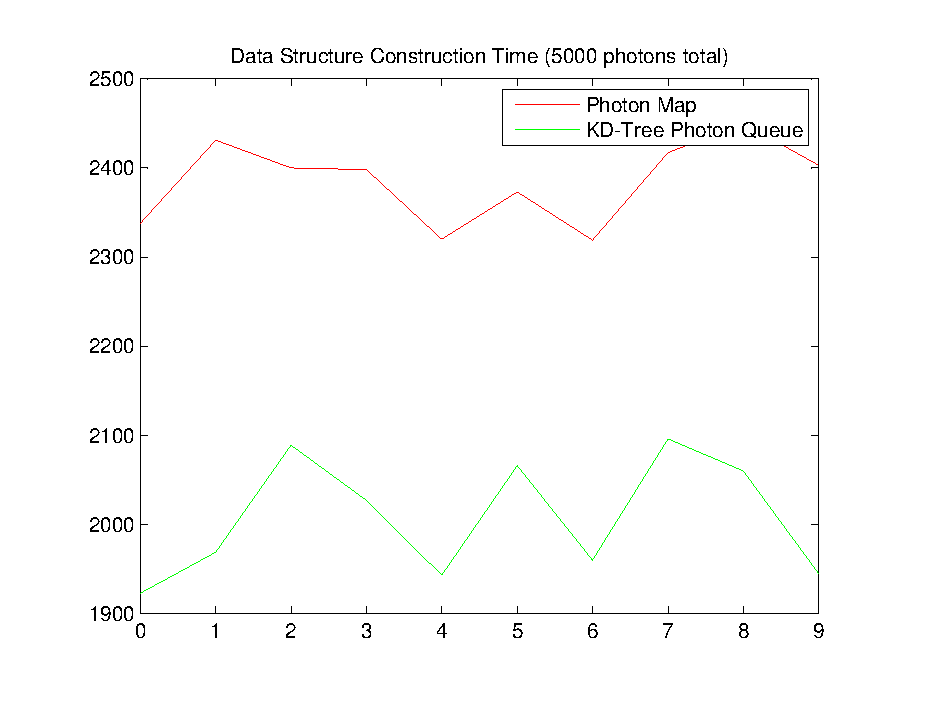
\includegraphics[width=\linewidth]{imgs/construction_time.pdf}}
    \renewcommand{\thefigure}{\thechapter.\arabic{figure}}
    \caption[]{Data structure construction time}
    \label{fig:construction_time} 
\end{figure} 

\section{Memory Consumption} 

The memory consumption is another important aspect we need to investigate. The memory capacity of the PC's video cards nowadays has been greatly extended, it is fairly easy to find an affordable video cards featured with 1024MB DDR5 on-board memory. However video memory is still a type of valuable resource. When analyzing the memory consumption of our technique compares to the brute force approach, we are looking at the data from two different running phases of our test program, the pre-rendering phase and rendering phase. 

As shown in figure \ref{fig:memory_consumption}, given the parameter of \emph{max frames} as \emph{10}, the memory consumption of our technique is considerably larger than the brute force, in fact, it requires more than 10 times more memory. The reason for this behavior is that we maintain a large buffer that works like circular buffer to keep track of all the photons data of previous frames, and the capacity of the buffer is determined by maximum number of frames we check back. In addition to the extra photon data, we also need to store another buffer on GPU memory that stores the photons that belongs to a kd-tree leaf node using photon indices which point to the photon data, buffer. Though the index is just represented with an 32-bit unsigned integer value which is much smaller than the detailed representation of a photon in the global buffer. 

\begin{figure}[ftp] 
    \centering 
    \fbox{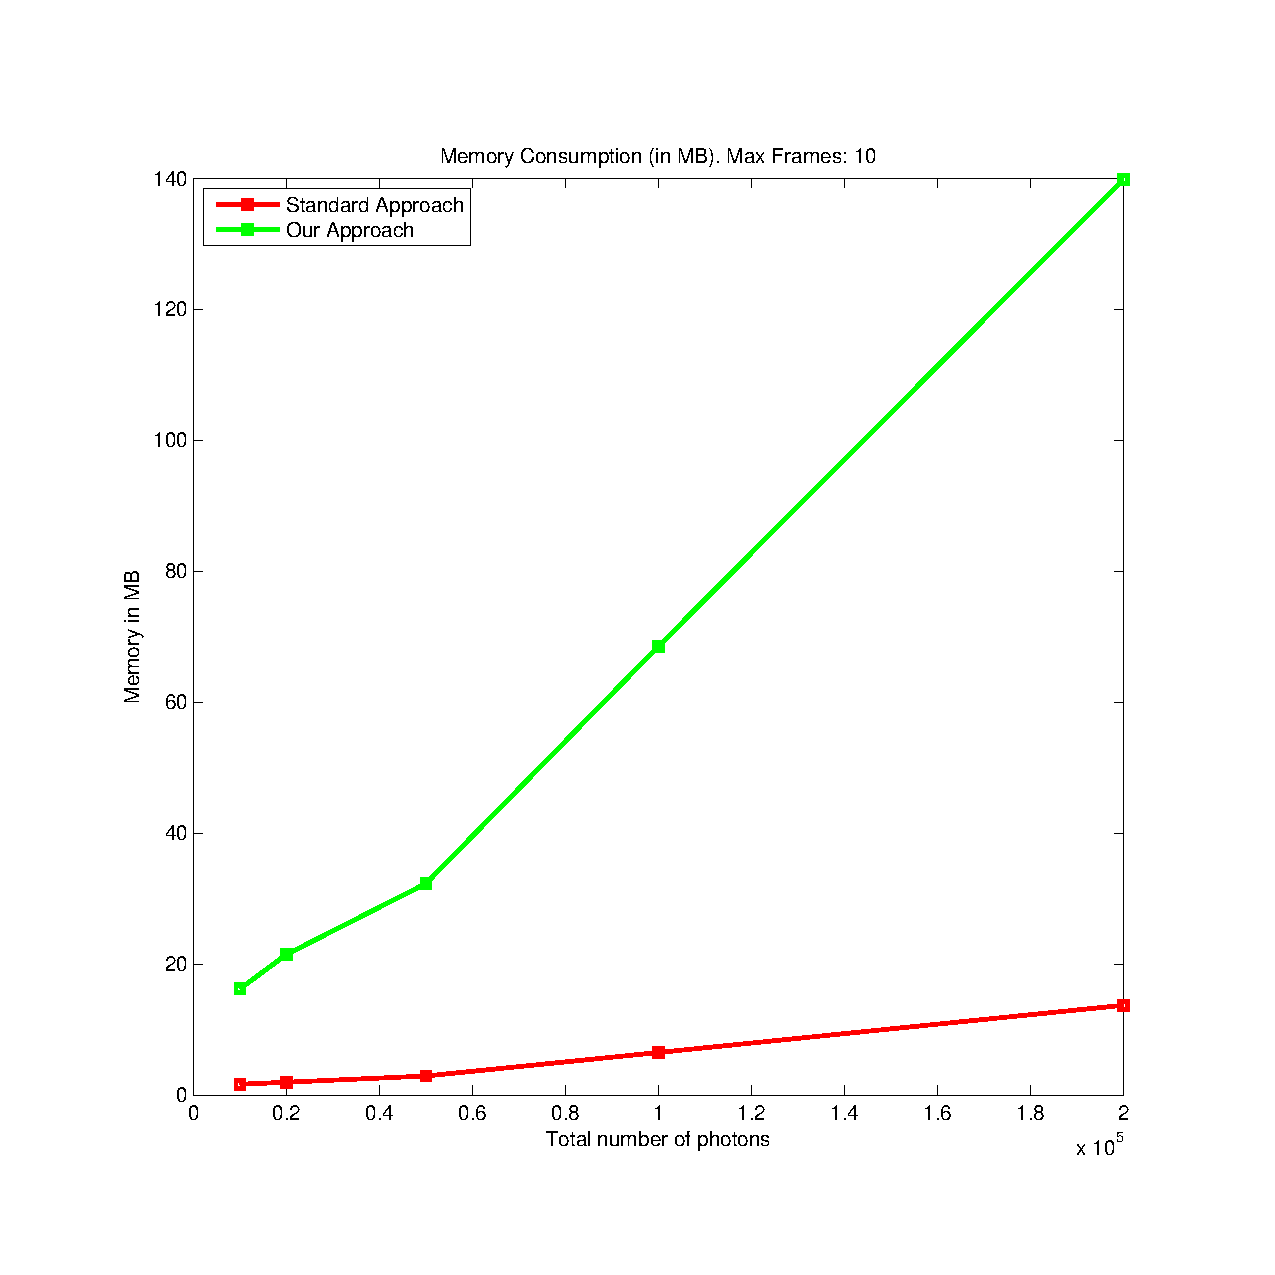
\includegraphics[width=\linewidth]{imgs/memory_consumption.pdf}}
    \renewcommand{\thefigure}{\thechapter.\arabic{figure}}
    \caption[]{Memory consumption in rendering phase.}
    \label{fig:memory_consumption} 
\end{figure}  

Although our new technique demands much more memory than the brute force does in the rendering phase, the memory requirement of our method is much lower than the brute force approach. This behavior is due to the big memory overhead introduced in kd-tree construction phase. Large amount of memory is allocated for the miscellaneous data structure such as the node list, the indices of triangles(triangles and points) and split list, and then will be released when construction is done. While our new technique does not require much temporary data. 

\begin{figure}[ftp] 
    \centering 
    \fbox{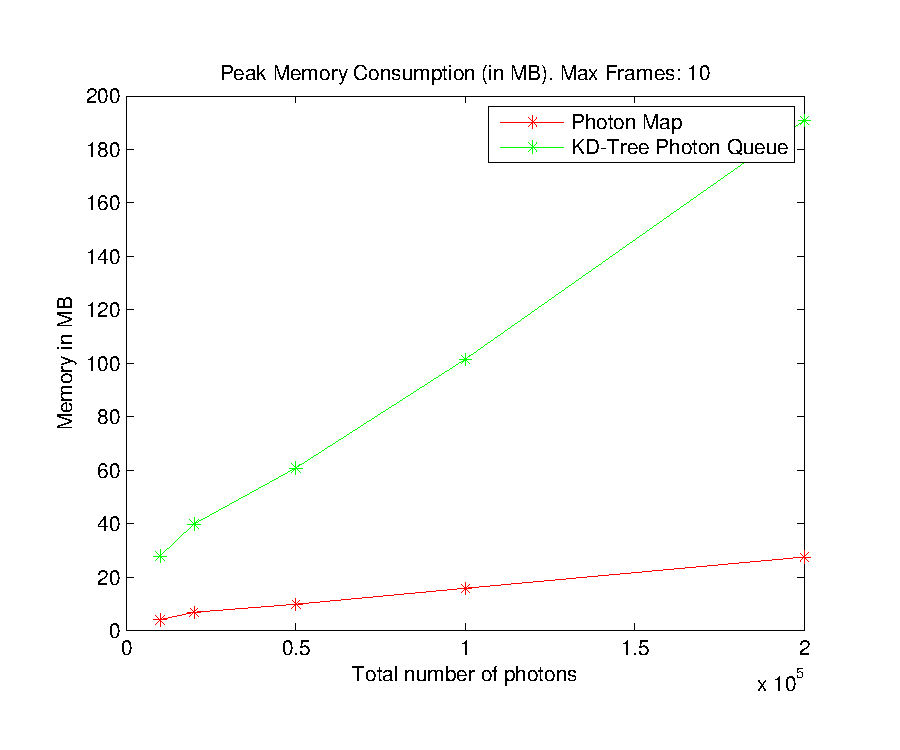
\includegraphics[width=\linewidth]{imgs/memory_consumption_2.pdf}}
    \renewcommand{\thefigure}{\thechapter.\arabic{figure}}
    \caption[]{Memory consumption in pre-render phase. }
    \label{fig:memory_consumption_2}  
\end{figure}   

As shown in figure \ref{fig:memory_consumption_2}, building a kd-tree for the photons demands much more memory than building the photons queue, even though the memory allocated here will release later, the peak memory consumption could bottleneck the performance of the whole program or even prevent the program from running for some video cards with smaller memory capacity. Since memory allocation is an expensive routine and kd-tree construction requires lots of temporary memory allocation/release, it becomes another important factor that brings negative impact on performance of the data structure construction for the brute force as we can see in the section \ref{sec:build_time}.  

\section{Photons Search}

In this section, we will show how the different techniques perform during the photon search. There are couple of parameters that have influence on the performance: 

\begin{itemize}

\item{The number of photons to search. }

\item{The search radius(maximum allowd distance between the query point and a photon). } 

\end{itemize} 

We will present how these parameters effect the photon search result and analyze the possible cause. 

\subsection{Number of Photons} 

As shown in the figure \ref{fig:photon_search_1}, the photon gathering of our technique is slightly faster than the standard photon mapping when number of photons is less than 150000, as the range of photons to search grows, it slows down and is out performed. As introduced earlier, our technique creates a buffer holding the photons that spatially belong to the leaf nodes of kd-tree for the scene objects, when performing the photon search, we traverse this built kd-tree with k-nearest neighbor algorithm to quickly reach the leaf nodes that is connecting with the photons that potentially fall into a pre-defined search range from the query point using the bounding box information of the kd-tree leaf nodes, then perform a linear search at this level. Compares to kd-tree built for the hundreds of thousands of photons in the scene, the kd-tree for geometry is usually far more coarse, especially for a relative simple scene. Therefore the kd-tree for a simple scene will have a small depth and a leaf node could have an large extent and holds a large number of photons. Thus the advantages of the binary search is out-weighted by the linear search. This is a possible reason why we have a result shown in figure \ref{fig:photon_search_1}. In an extreme case, when there is no split in the scene, thus the kd-tree only have one node, the root node which contains everything, the photon search will be degenerated into a linear search. 

\begin{figure}[ftp] 
    \centering 
    \fbox{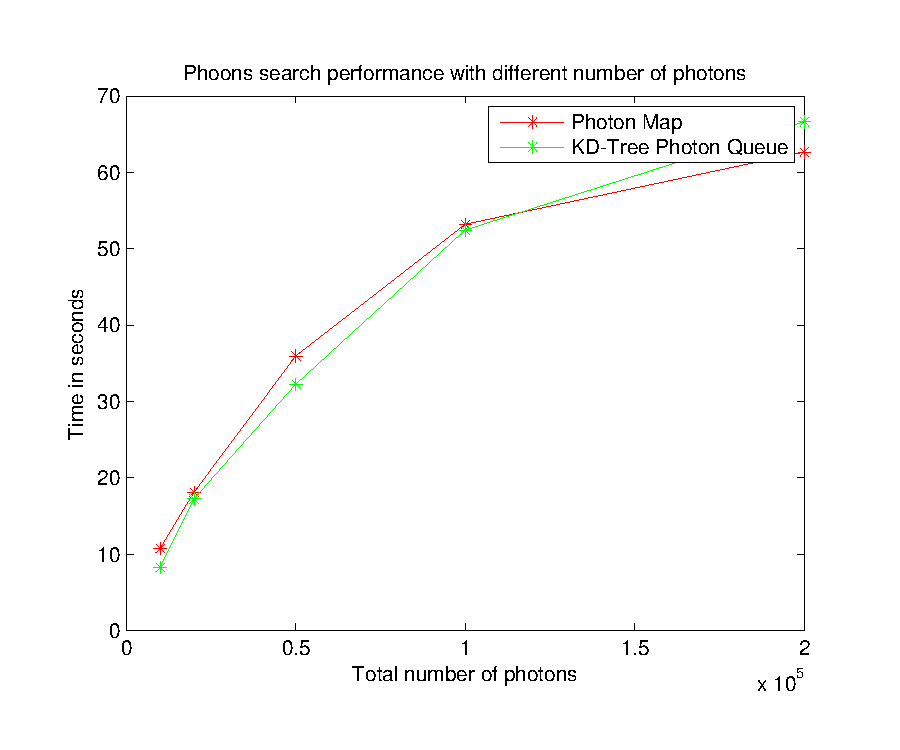
\includegraphics[width=\linewidth]{imgs/photon_search_1.pdf}}
    \renewcommand{\thefigure}{\thechapter.\arabic{figure}}
    \caption[]{Photon search performance with different number of photons. }
    \label{fig:photon_search_1}  
\end{figure} 

\subsection{Query Radius}

Figure \ref{fig:photon_search_2} shows that how the query radius effect the photon search performance. The standard photons search algorithm and our technique both have an almost steady increase in search time with an increasing query radius. For standard photon mapping method, since more kd-tree node will be enqueued to the stack waiting to be visited as the query radius increases, this brings larger kd-tree traversal overhead. When using photons queue for range search, the lost of performance becomes less than the standard photon mapping. As explained earlier, more photons are associated with one kd-tree leaf nodes, thus there are less nodes pushed to the local stack and the overhead of traversing the kd-tree is avoided. 

\begin{figure}[ftp] 
    \centering 
    \fbox{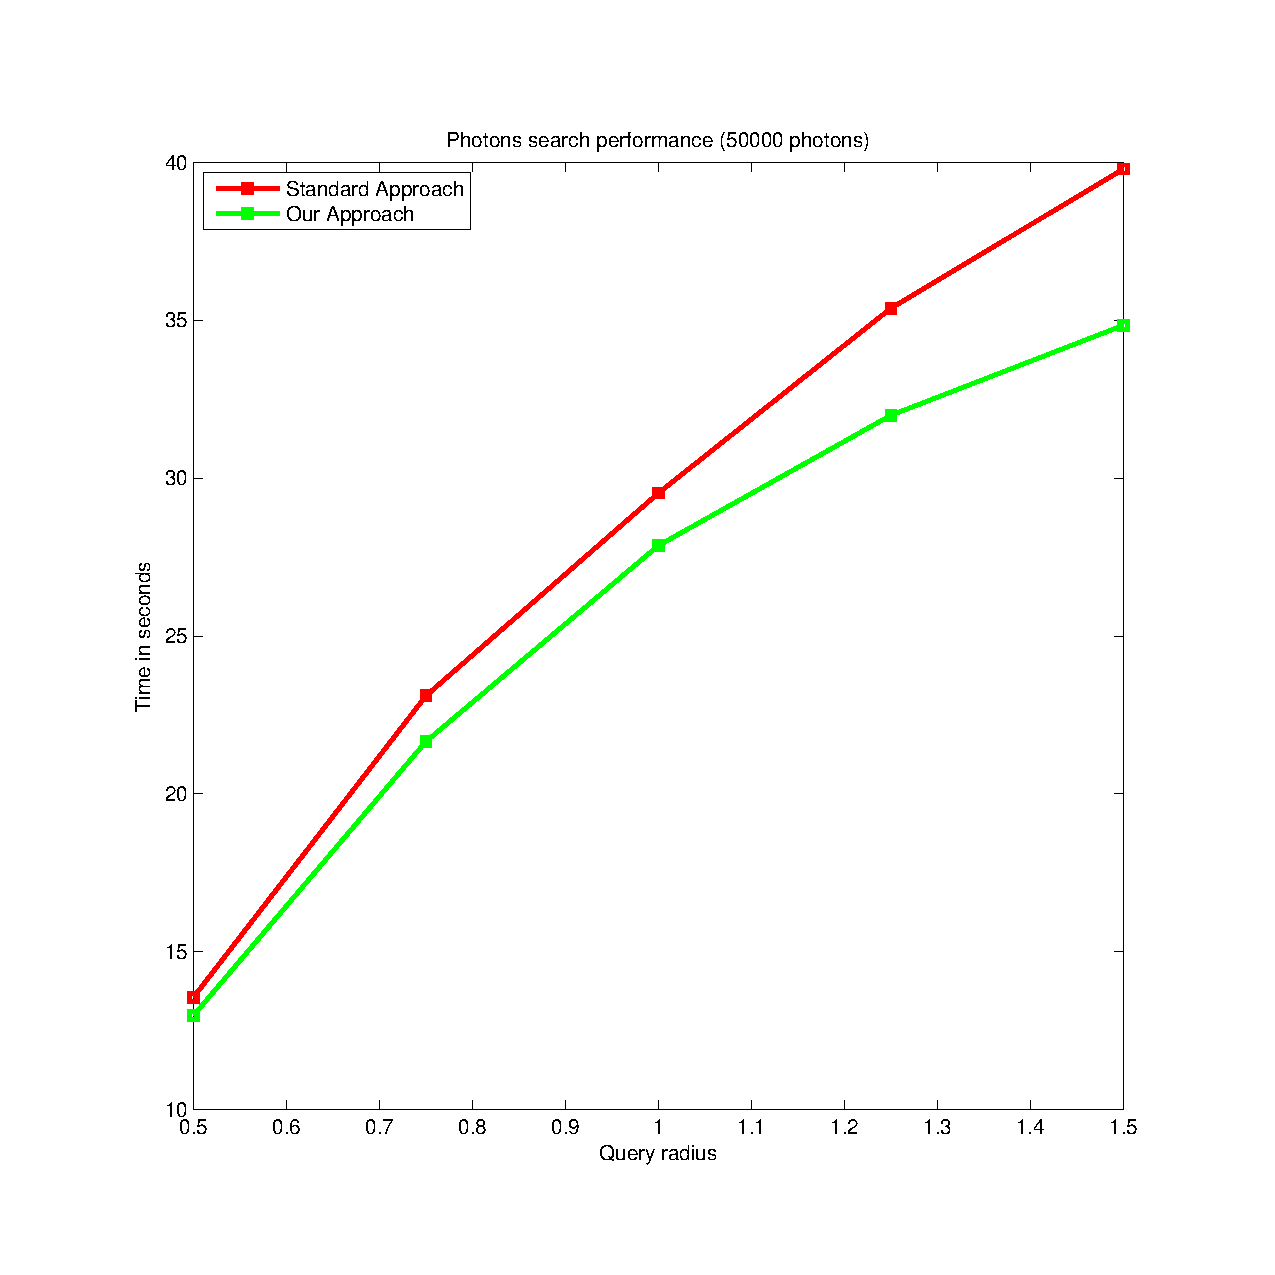
\includegraphics[width=\linewidth]{imgs/photon_search_2.pdf}}
    \renewcommand{\thefigure}{\thechapter.\arabic{figure}}
    \caption[]{Photon search performance with different query radius. }
    \label{fig:photon_search_2}  
\end{figure} 

\section{Image Quality}

In this section we take a look at the quality of our approach. As described in chapter 3, our new approach uses an incremental scheme to update the kd-tree and photons queue for the rendering to be beneficial for the dynamic scene with moving light source. Therefore it makes more sense to look at the result images of a range of frames to see the image quality, the light source will also be moving in the frame sequence so that we can see the change of equilibrium distribution of radiance in the scene. To obtain a better knowledge on how the photons are distributed in the scene each frame, we will present the photons visualization result images as well along with the result image. 

Several key parameters defined in our experiments for both the standard photon mapping method and our new approach are presented in the table \ref{tab:expr_params}. 

\begin{table}[ht]
\begin{center}
	
	\renewcommand{\arraystretch}{1.2}
	\begin{tabular}{p{5cm}p{3cm}p{5cm}}
	
	Parameter  				& 		Default Value 		&		Description \\ 
	
	\hline 

	Max. Photons Bounces		& 		3					&		The maximum photons reflection will be traced. \\  

	\hline 					

	Total Number of Photons 	& 		200000				&		The total number of photons emitted from the light 																	source. \\

	\hline

	Light Source Type			& 		Point Light			& 		The type of light source, point light and area light
																are supported. However in this experiments only point 																	light is used. \\ 
	
	\hline
	
	Light Source Position 		& 	 	(0.0, 10.0, 0.0)		&		Default light source position in the scene. \\  


	\hline 
	
	Light Emission Intensity	&		(1.0, 1.0, 1.0)		&		The RGB representation of light emitted radiance.\\  

	\hline 

	Maximum Frames Counter 	& 		10 					& 		The maximum number of frames we keep track of. Given 																	the total number of photons as 200000, the photons 																	emitted for each frame is 20000\\

	\hline
	
	Image Resolution 			&		512 x 512				&		The resolution of result image. \\

	\hline 
	
	Samples per Pixel			& 		1 					& 		Multi-sampling is not used in the experiments thus 																	there is only 1 ray being traced per pixel.\\
	
	\hline 
	
	Trace Shadow Rays			&		Off					& 		Toggle tracing the shadow rays. \\

	\hline

	Specular Reflection		&		Off					&		Toggle of specular reflection when tracing photons. \\

	\hline
	
	\end{tabular}
\end{center} 
\caption{Experiments Parameters}
\label{tab:expr_params}
\end{table}

In figure \ref{fig:pm_global}, we firstly present the result image rendered with default values of the parameters listed in table \ref{tab:expr_params} using standard photon mapping algorithm and phtons visualization image. 

\begin{figure}[htp] 
\begin{center}
    \fbox{
	\subfigure[Test subfigure 1]{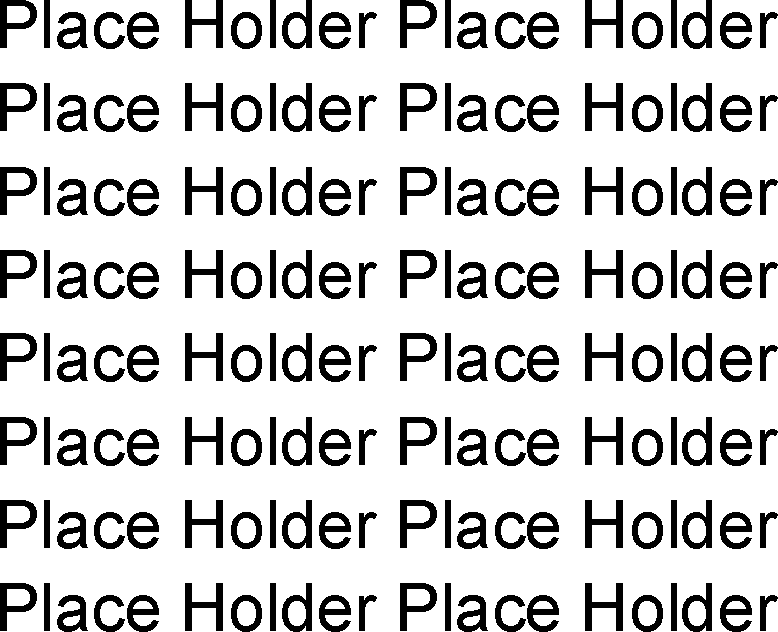
\includegraphics[scale=0.5]{imgs/place_holder.pdf}}
	\subfigure[Test subfigure 2]{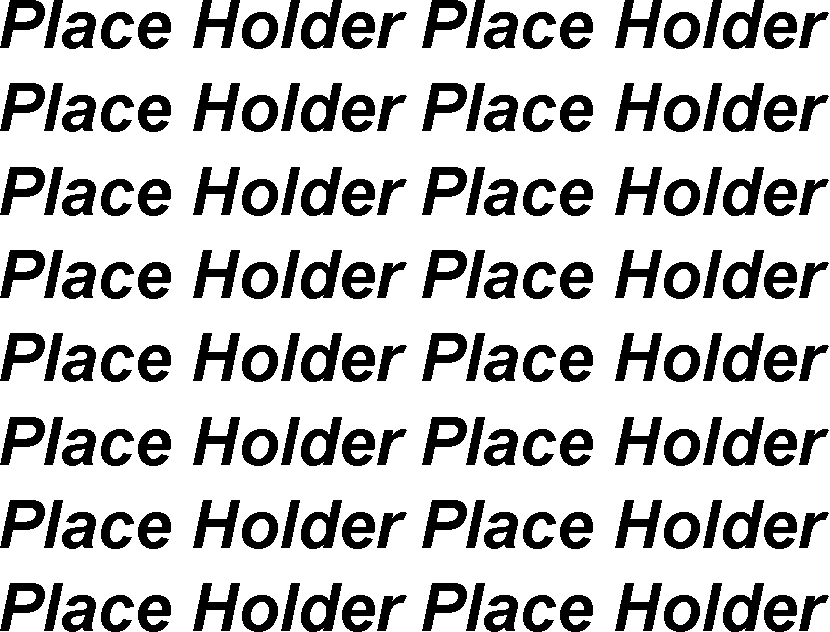
\includegraphics[scale=0.5]{imgs/place_holder_2.pdf}}
	}
    \renewcommand{\thefigure}{\thechapter.\arabic{figure}}
    \caption[]{Memory consumption in rendering phase.}
    \label{fig:pm_global} 
\end{center} 
\end{figure}   

The following series of images groups rendered with our new approach is a frame sequence rendering a scene with moving point light source. The figure \ref{fig:pq_frame_1} frame is rendered with the point light located in the default position.  

\begin{figure}
\label{fig:result_images1}
\begin{center}
\setlength{\tabcolsep}{0mm}
\subfigure[]{%	Result Image
\begin{tabular}{c}
\includegraphics*[scale=0.25]{imgs/pq_frame0.pdf}\\
\includegraphics*[scale=0.25]{imgs/pq_frame1.pdf}\\
\includegraphics*[scale=0.25]{imgs/pq_frame2.pdf}\\
\includegraphics*[scale=0.25]{imgs/pq_frame3.pdf}
\end{tabular}
}%
\subfigure[]{%	Photons Visualization
\begin{tabular}{c}
\includegraphics*[scale=0.25]{imgs/pqv_frame0.pdf}\\
\includegraphics*[scale=0.25]{imgs/pqv_frame1.pdf}\\
\includegraphics*[scale=0.25]{imgs/pqv_frame2.pdf}\\
\includegraphics*[scale=0.25]{imgs/pqv_frame3.pdf}
\end{tabular}
}%
\caption{a caption}
\end{center}

\end{figure}

\begin{figure}
\begin{center}
\setlength{\tabcolsep}{0mm}
\subfigure[]{%	Result Image
\begin{tabular}{c}
\includegraphics*[scale=0.25]{imgs/pq_frame4.pdf}\\
\includegraphics*[scale=0.25]{imgs/pq_frame5.pdf}\\
\includegraphics*[scale=0.25]{imgs/pq_frame6.pdf}\\
\includegraphics*[scale=0.25]{imgs/pq_frame7.pdf}
\end{tabular}
}%
\subfigure[]{%	Photons Visualization
\begin{tabular}{c}
\includegraphics*[scale=0.25]{imgs/pqv_frame4.pdf}\\
\includegraphics*[scale=0.25]{imgs/pqv_frame5.pdf}\\
\includegraphics*[scale=0.25]{imgs/pqv_frame6.pdf}\\
\includegraphics*[scale=0.25]{imgs/pqv_frame7.pdf}
\end{tabular}
}%
\caption{a caption}
\end{center}
\label{fig:result_images2}
\end{figure}

\begin{figure}
\begin{center}
\setlength{\tabcolsep}{0mm}
\subfigure[]{%	Result Image
\begin{tabular}{c}
\includegraphics*[scale=0.25]{imgs/pq_frame8.pdf}\\
\includegraphics*[scale=0.25]{imgs/pq_frame9.pdf}
\end{tabular}
}%
\subfigure[]{%	Photons Visualization
\begin{tabular}{c}
\includegraphics*[scale=0.25]{imgs/pqv_frame8.pdf}\\
\includegraphics*[scale=0.25]{imgs/pqv_frame9.pdf}
\end{tabular}
}%
\caption{a caption}
\end{center}
\label{fig:result_images3}
\end{figure}

As shown in figure \ref{fig:brdf}, figure \ref{fig:result_images2} and figure \ref{fig:result_images3}, the quality of 	result images become better and finally stable after a certain number of frames. It is not difficult to understand why we have such result according to our algorithm, as we trace fewer photons for each frame, the beginning few images apparently are less illuminated by the light source, in the following frames, we keep shooting and more photons into the scene and accumulating the photons to the photons queue. Therefore we can visualize more and more photons and the scene becomes brighter. The number of photons in the scene will become stable when the maximum frames, since there are same amount of photons traced as they are supposed to be compares to the standard approach. Eventually we will achieve same image quality as of the standard photon mapping. 




%-------------------------
% Chapter 5: Result and Analysis 	(~18	 p)
\chapter{Conclusions}

%\section{Conclusions}
In this research, we mainly focus on developing an improved photon mapping technique specifically for current generation GPU taking the advantage of the massive parallelized computation power. We started with introducing the theoretic basis of global illumination, then we reviewed the existing approaches published on the solving the problem, especially the photon mapping techniques exploited the parallelism with GPU. In our opinion, the existing method suffers from a deficiencies in how it handles the dynamic scene. After analyzing the weakness, we present a new approach trying to avoid another kd-tree construction exclusively for photon data and support an incremental updating scheme by associating the photons data with the kd-tree of the geometric objects and accumulating the photons from previous frames for K Nearest Neighbor photon searching. To proof our concept we implemented the test programs for both the existing and our new approach and carried out a series of benchmarks.

% TF: Add a brief point-form summary of what is new/different about your approach.

In our tests we observed that our approach was faster during construction and almost all the photon search tests among certain range of frames for a dynamic scene. Especially the construction time was greatly reduced compared to the old approach. Along with speed measurements, we also examined the memory consumption of both approaches. Our approach consumes more memory in rendering phase since the photon data from previous frames. But the memory consumption in the construction phase is much less than the existing method. Because we only require the construction of kd-tree for the scene. The memory consumption also strongly depends on the number of frames we want to store for the photons. Finally, we validate the quality of the rendered by directly visualizing the photons in the scene.

\section{Future Work}

We believe that there are a couple of interesting topics the future work can work on to improve our new approach. The first one is improve the algorithm of the classifying the photons to the kd-tree's leaf nodes to achieve more efficient parallelization. The current solution is that each thread works on one leaf node iterating over all the photons, this could lead considerable deficiency of parallelization on GPU especially when the height of the tree is relative low (there are less leaf nodes) due to the low occupancy of CUDA threads. One possible solution is to map the photons to CUDA threads instead, marking the photons that belong  to certain kd-tree leaf node and applying a parallel primitive algorithm such as compact to calculate the indices of photons for each kd-tree leaf node in parallel.

Another interesting application we can explore further is to test and observe that how participating media such as smoke, dust or clouds effect the performance using our approach. The participating media will affect light when it travels through them, the light beam is either absorbed or scattered. Since our approach spatially encodes the distribution of the photons based on the volume boundary of the kd-tree nodes, we think our approach is suitable for storing photon information of volumetric participating media and good performance could be expected.

In addition to keep evolving the approach algorithmically, we certainly cannot ignore the impact brought by the developments in graphics hardware on the photon mapping techniques. With the latest generation of GPUs and development framework, the applications will benefit from better GPU performance and more flexibility, such as better performance for non-coalesced memory access implicit hardware optimizations which is almost free for developers. 	

%o-------------------------
% Chapter 6: Conclusion		(~2 p)
\include{ch6}		

%-------------------------
% Appendix 
%\chapter{Appendix}				
%-------------------------

%\bibliography{C:/Users/lenovo/thesis/working/thesis/bib/refdb}                         %place your .bib files here
%\bibliographystyle{ieeetr}               %the bibliography style to use
%\bibliography{refdb}

\end{document}
